\chapter{测试平台硬件架构}
\label{cha:Hardware}

\section{平台选型}

我们选用Nvidia Jetson NANO(如图~\ref{fig:Jetson-Nano})作为主要的开发平台,NVIDIA Jetson Nano开发人员工具包是一台功能强大的小型计算机,可并行运行多个神经网络,以用于图像分类,对象检测,分段和语音处理等应用,该平台的功耗仅为5瓦。

\begin{figure}[htbp] % use float package if you want it here
    \centering
    \includegraphics[height=6cm]{Jetson-Nano.jpg}
    \caption{Nvidia Jetson NANO}
    \label{fig:Jetson-Nano}
\end{figure}

初步的硬件平台,采用无线局域网通信,图~\ref{fig:wifi}为将AC8265和片状5GHz天线装到Jetson Nano Developer Kit上。

\begin{figure}[htbp]
    \begin{minipage}{0.48\textwidth}
      \centering
      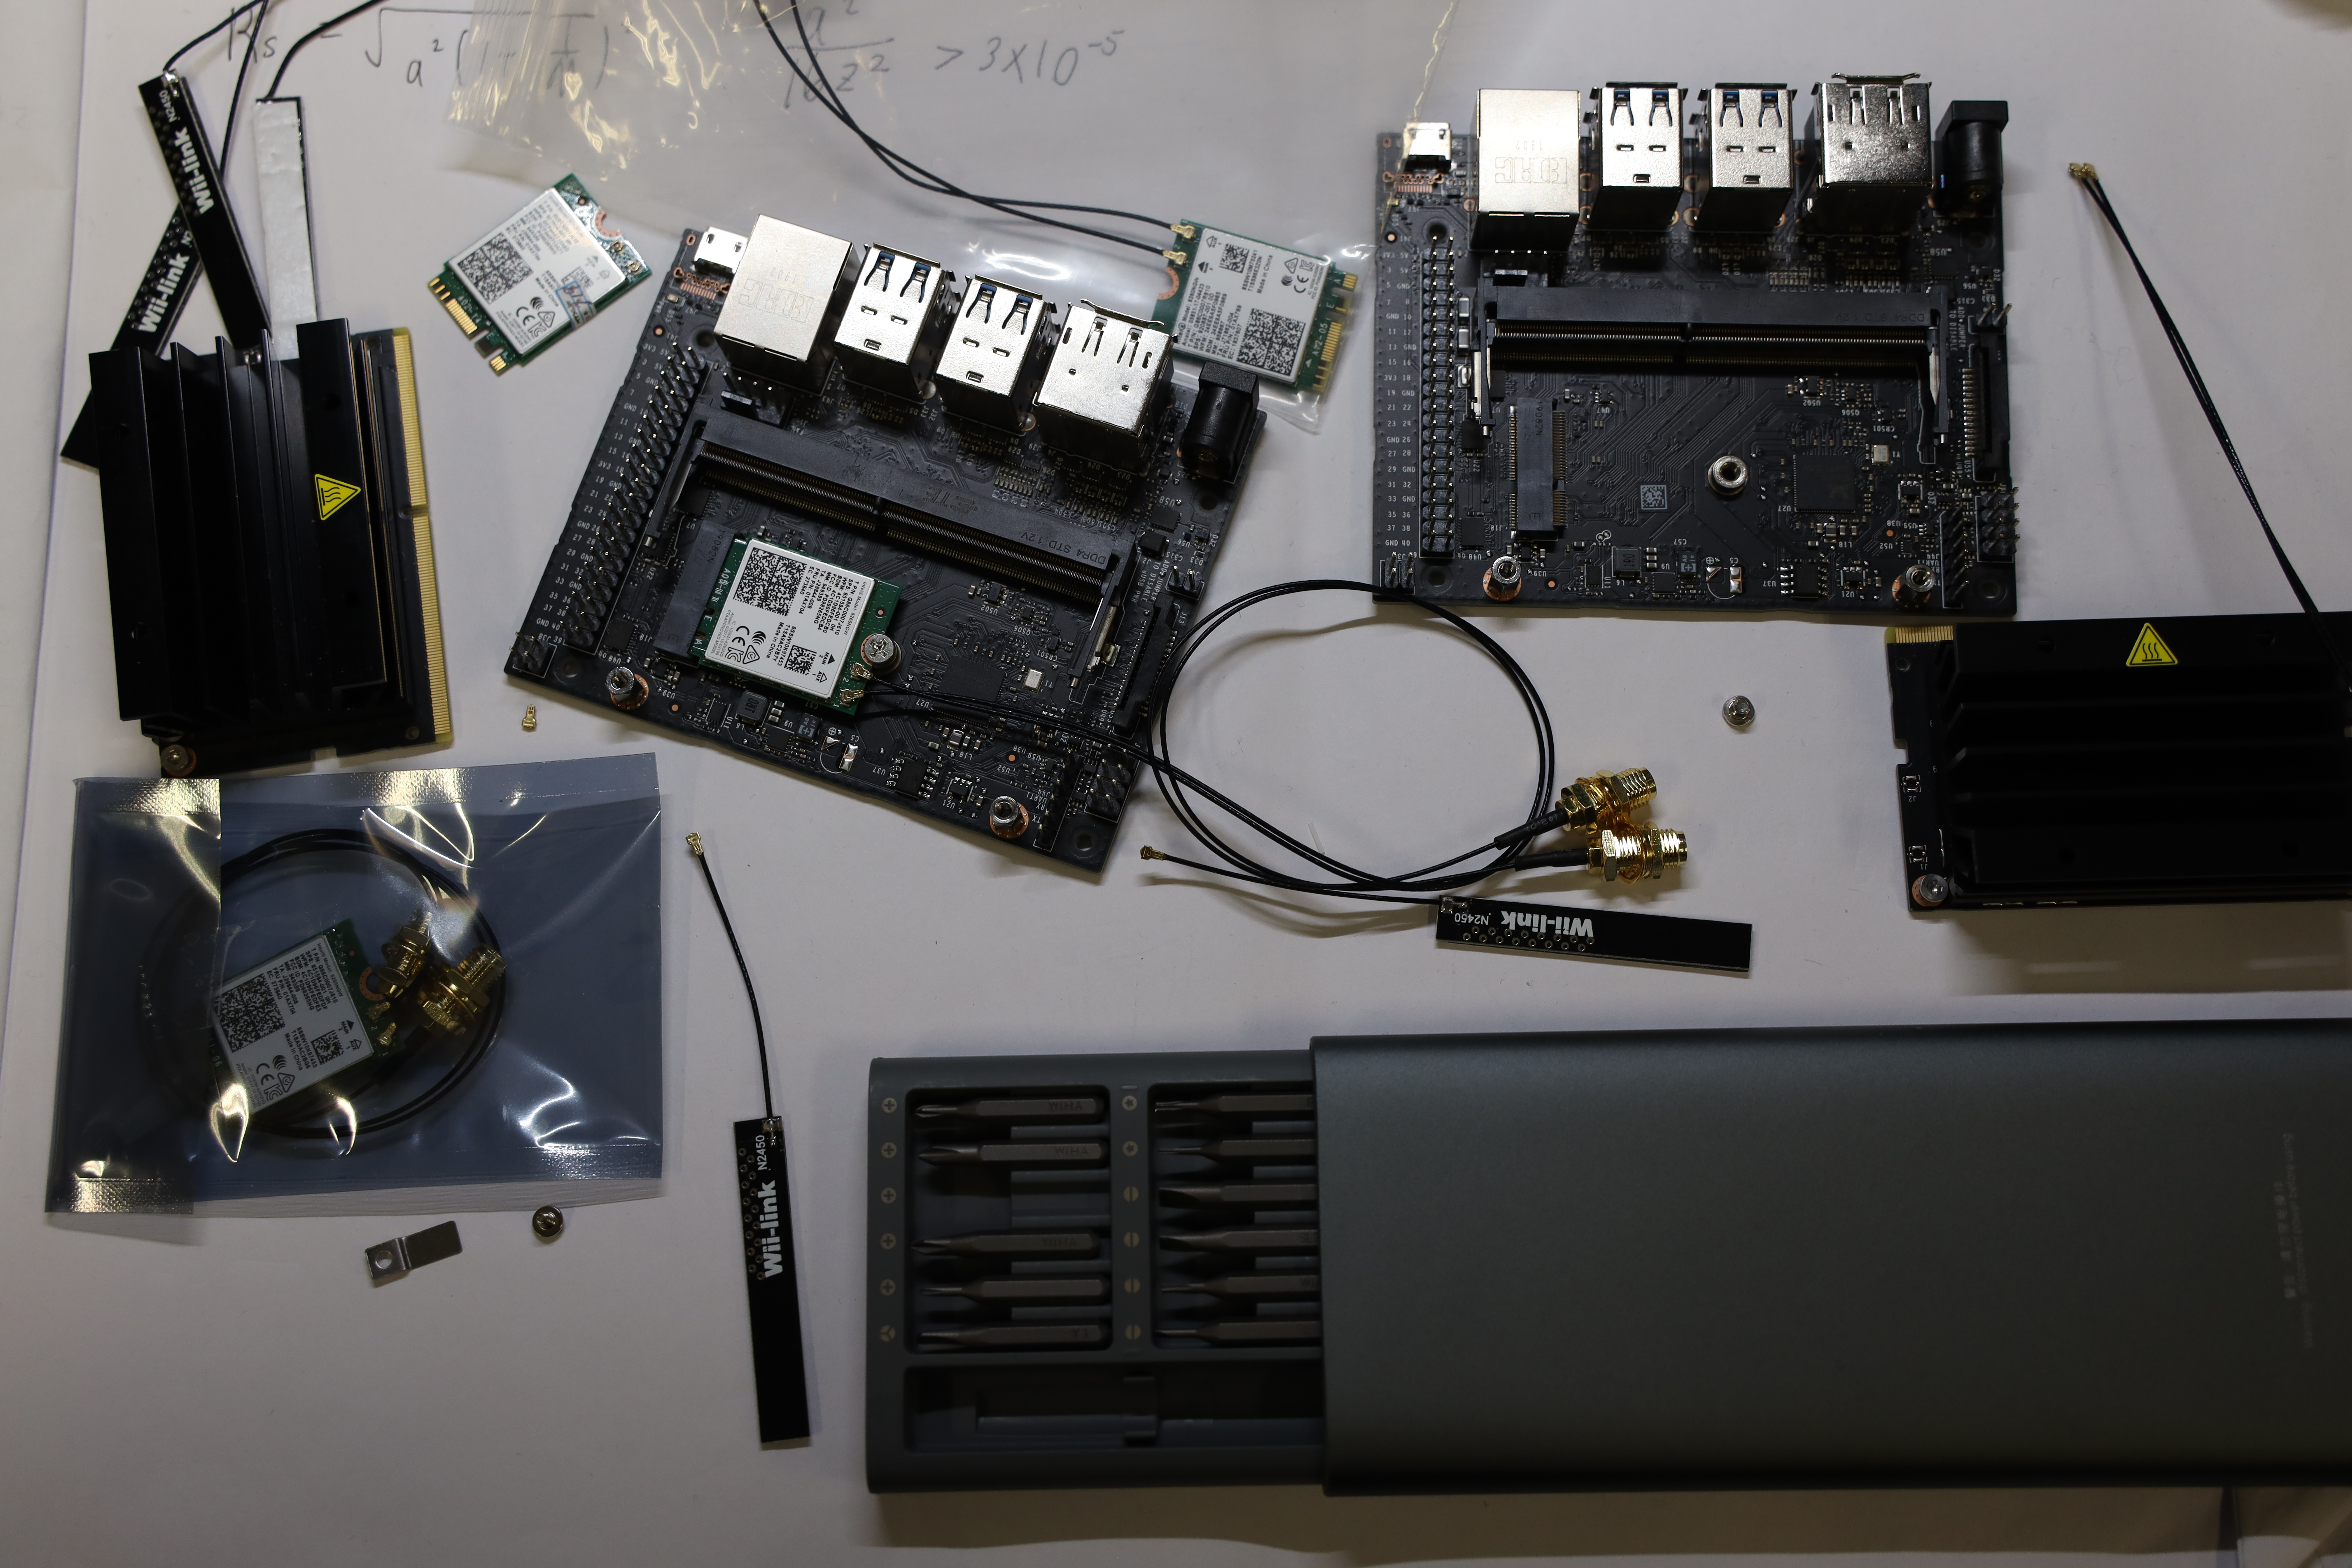
\includegraphics[height=5cm]{DA4A3052.JPG}
      \caption{为Nano添加无线网功能}
      \label{fig:wifi}
    \end{minipage}\hfill
    \begin{minipage}{0.48\textwidth}
      \centering
      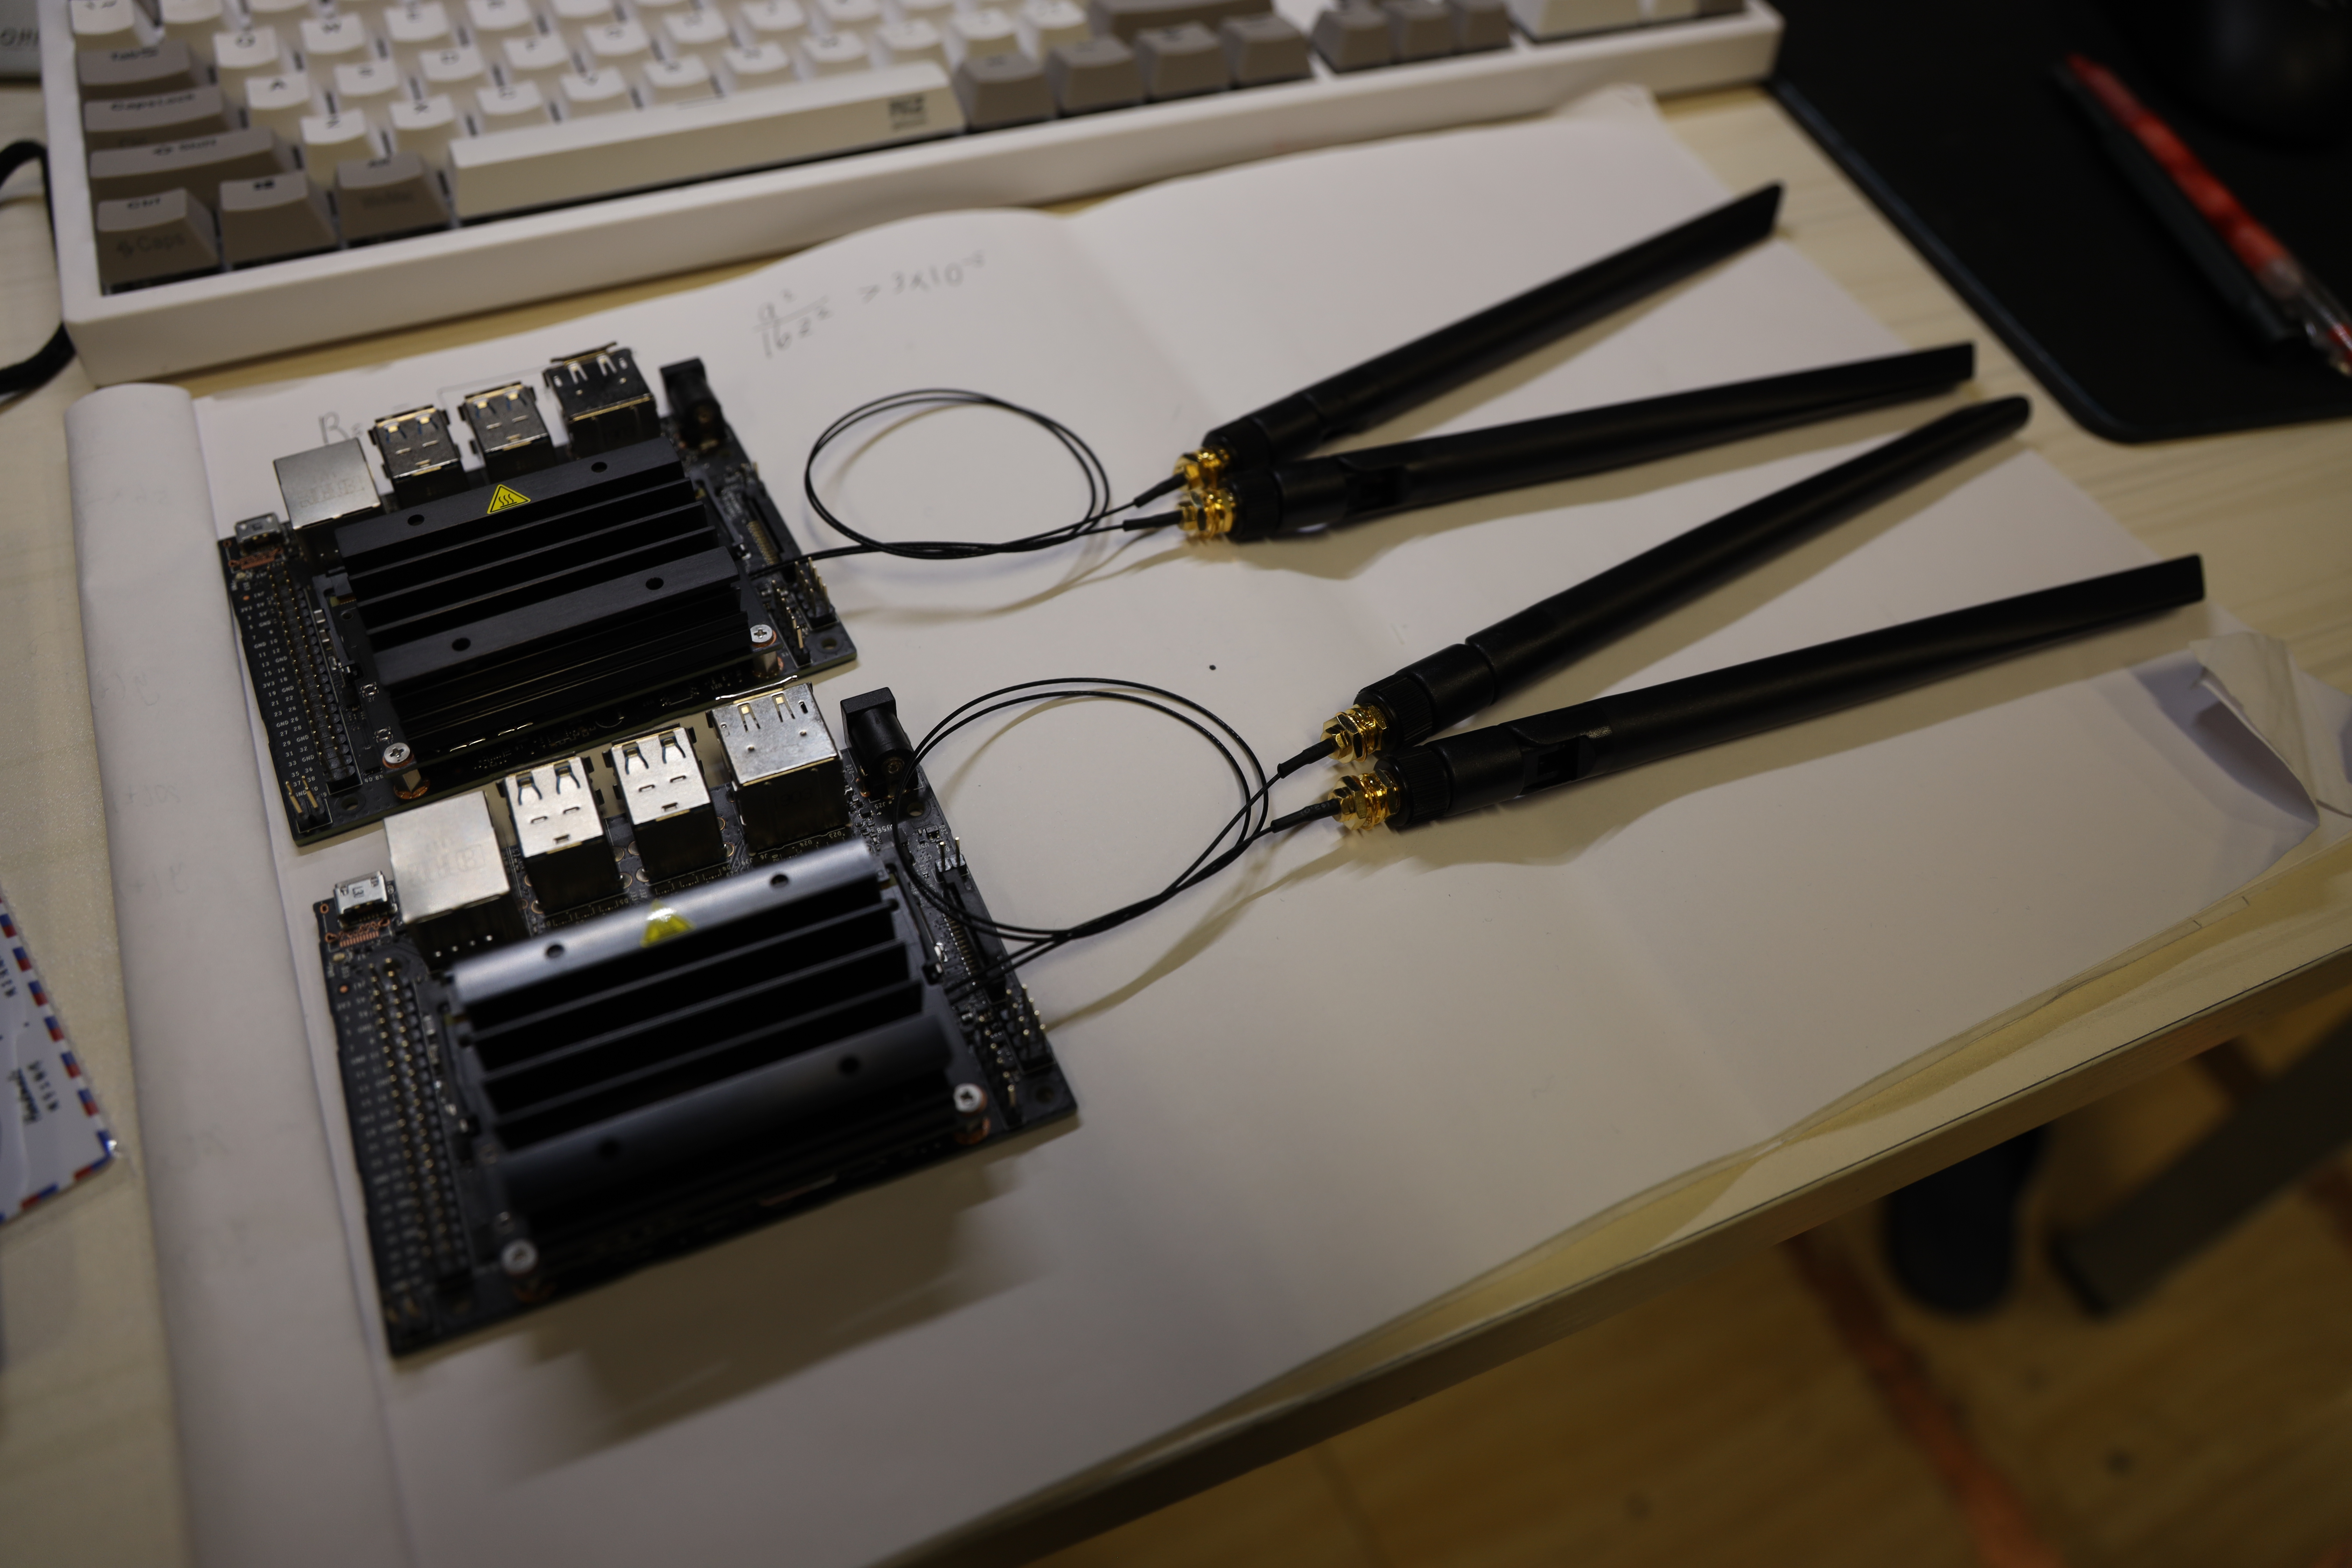
\includegraphics[height=5cm]{DA4A3066.JPG}
      \caption{两机组通信测试平台}
      \label{fig:two-setup}
    \end{minipage}
\end{figure}


\section{电机和全向轮配置}

尝试多种电机与全向轮的配合方式,寻找最优方案:

同样体积的直流减速电机的扭矩比步进电机要大,拥有编码器的电机(如图~\ref{fig:Motor-1})能够反馈实时转速,从而可以使用PID控制进行控制;带有蜗杆的电机(如图~\ref{fig:Motor-2})可以缩小底盘面积,但蜗杆传动使得动力传输方向不可逆,即无法通过转动轮子带动电机转动,这使得手动推动平台变得困难、不顺滑;反折的N20电机(如图~\ref{fig:Motor-3})同样可以缩小底盘面积,但不带编码器的情况下电机尾部就已经和轮子摩擦,在联轴器完全紧固的情况下无法正常工作。

\begin{figure}[htbp]
  \begin{minipage}{0.31\textwidth}
    \centering
    \includegraphics[height=4cm]{Motor-1.jpg}
    \caption{N20减速电机(带编码器)}
    \label{fig:Motor-1}
  \end{minipage}\hfill
  \begin{minipage}{0.31\textwidth}
    \centering
    \includegraphics[height=4cm]{Motor-2.jpg}
    \caption{N20减速电机(带蜗杆)}
    \label{fig:Motor-2}
  \end{minipage}\hfill
  \begin{minipage}{0.31\textwidth}
    \centering
    \includegraphics[height=4cm]{Motor-3.jpg}
    \caption{N20减速电机(反折)}
    \label{fig:Motor-3}
  \end{minipage}
\end{figure}

步进电机无需编码器即可控制当前电机的角度,我们考虑体积较小的两相四线微型步进电机:反折的步进电机(如图~\ref{fig:Motor-Step-1})可以缩小底盘面积,另外还有两种不同大小和扭矩的直线步进电机(如图~\ref{fig:Motor-Step-2}和图~\ref{fig:Motor-Step-3})。

\begin{figure}[htbp]
  \begin{minipage}{0.31\textwidth}
    \centering
    \includegraphics[height=4cm]{Motor-Step-1.jpg}
    \caption{反折的微型步进电机}
    \label{fig:Motor-Step-1}
  \end{minipage}\hfill
  \begin{minipage}{0.31\textwidth}
    \centering
    \includegraphics[height=4cm]{Motor-Step-2.jpg}
    \caption{微型步进电机(小)}
    \label{fig:Motor-Step-2}
  \end{minipage}\hfill
  \begin{minipage}{0.31\textwidth}
    \centering
    \includegraphics[height=4cm]{Motor-Step-3.jpg}
    \caption{微型步进电机(大)}
    \label{fig:Motor-Step-3}
  \end{minipage}
\end{figure}